%!TEX root = ../thesis.tex

\chapter{Evaluation and Discussion}
\label{ch:eval}

This chapter presents the outcomes of test executions and compare it to the original Java COMER framework implementation, as well as to CT approach. For this research, I formulated following research questions:

\begin{itemize}
  \item \textbf{RQ1:} How does the COMER framework compare to traditional Combinatorial Testing (CT) methods in terms of test case generation efficiency?
  \item \textbf{RQ2:} Can COMER be used to identify vulnerabilities in complex cybersecurity software more effectively than traditional CT methods?
  \item \textbf{RQ3:} Can this integrated technique be standardized into a framework or toolset for automated security testing?
  \item \textbf{RQ4:} Can relevant metamorphic relations and test pairs be systematically generated for complex cybersecurity software? Or does it require domain expertise?
\end{itemize}

\section{Evaluation}
\label{sec:evaluation}

To evaluate the efficacy of my implementation of the COMER framework, I conducted a series of experiments comparing its performance with the original Java implementation by Niu \textit{et al.} \cite{comer}.
The experiments focused on assessing the framework's ability to generate test cases accurately and efficiently across various scenarios.

Charts below present the results of the experiments conducted on the COMER framework. The experiments were conducted on the following injection types: SQL Injection on DVWA, SQL Injection on Web Goat, Blind SQL Injection on  Web Goat, and Form Sanitization in login forms. The injection were selected based on the large potential number of errors that could be uncovered and the complexity of the injection, including MR complexity and the number of test cases generated. Also, I choose to include Quicksort as a target for testing because original paper used it in its evaluation. All targets are described in Table~\ref{fig:injections}.

For the SQL injections I used Metamorphic Relations (MRs) to generate test cases. The MRs were designed to simulate various injection attack scenarios, such as UNION injections, where we try to add additional rows to the resulting SELECT, Condition injections, where we try to modify condition check to always be True, and string escape, there we specifically try to escape strings. All of the relations were used to either add a constant to input or reverse some part of the input.

The results are shown in the three charts, presenting number of test cases generated in Fig.~\ref{fig:test_cases}, number of faults detected in Fig.~\ref{fig:faults}, and execution time in seconds in Fig.~\ref{fig:exec_time}. The results are considered for three different scenarios: COMER with 75\% probability of selecting MR approach, COMER with 50\% probability of selecting MR approach, COMER with 25\% probability of selecting MR approach, and traditional CT approach using AllPairs algorithm. The selection of such scenarios allows to evaluate the difference between the traditional CT approach and the COMER framework, as well as the impact of the MR approach selection probability on the results.

\begin{table}[htbp]
  \centering
  \caption{Target Descriptions}
  \begin{tabular}{lrrr}
    \toprule
    Target & Domain size & MRs & Vulnerabilities \\
    \midrule
    Quicksort & $3^6$ & $3$ & $0$ \\
    SQL DVWA & $2^8*3*5*8$ & $3$ & $6$ \\
    SQL Web Goat & $2^7*6*10$ & $3$ & $6$ \\
    SQL Blind Web Goat & $2^7*6*10$ & $3$ & $6$ \\
    Form Sanitization & $2^{11} * 4^2$ & $2$ & $3$ \\
    \bottomrule
  \end{tabular}
  \label{fig:injections}
\end{table}

\begin{figure}[!t]
    \centering
    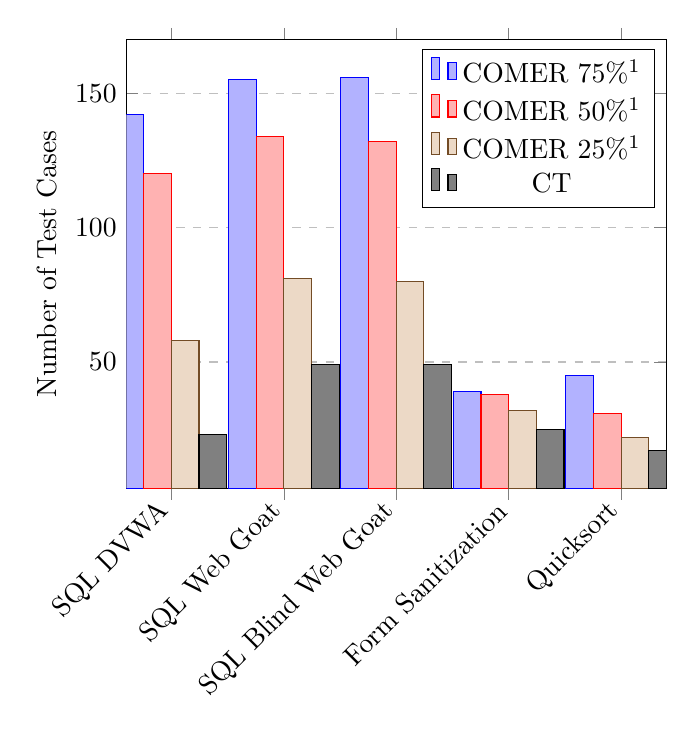
\begin{tikzpicture}
        \begin{axis}[
            ylabel={Number of Test Cases},
            ybar=0pt,
            bar width=10pt,  % Adjusts th;e gap between bar groups
            ymajorgrids=true,
            grid style=dashed,
%             legend pos=north west,
            symbolic x coords={SQL DVWA, SQL Web Goat, SQL Blind Web Goat, Form Sanitization, Quicksort},
            xtick=data,
            x tick label style={rotate=45, anchor=east},
        ]

        \addplot coordinates {
            (SQL DVWA, 142)
            (SQL Web Goat, 155)
            (SQL Blind Web Goat, 156)
            (Form Sanitization, 39)
            (Quicksort, 45)
        };
        \addlegendentry{COMER 75\%$^1$}

        \addplot coordinates {
            (SQL DVWA, 120)
            (SQL Web Goat, 134)
            (SQL Blind Web Goat, 132)
            (Form Sanitization, 38)
            (Quicksort, 31)
        };
        \addlegendentry{COMER 50\%$^1$}

        \addplot coordinates {
            (SQL DVWA, 58)
            (SQL Web Goat, 81)
            (SQL Blind Web Goat, 80)
            (Form Sanitization, 32)
            (Quicksort, 22)
        };
        \addlegendentry{COMER 25\%$^1$}


        \addplot coordinates {
            (SQL DVWA, 23)
            (SQL Web Goat, 49)
            (SQL Blind Web Goat, 49)
            (Form Sanitization, 25)
            (Quicksort, 17)
        };
        \addlegendentry{CT}

        \end{axis}
    \end{tikzpicture}
    \caption{Number of Test Cases generated for Different Injection Types. $^1$Percentage Corresponds to probability that MR approach will be selected.}
    \label{fig:test_cases}
\end{figure}

\begin{figure}[!t]
    \centering
    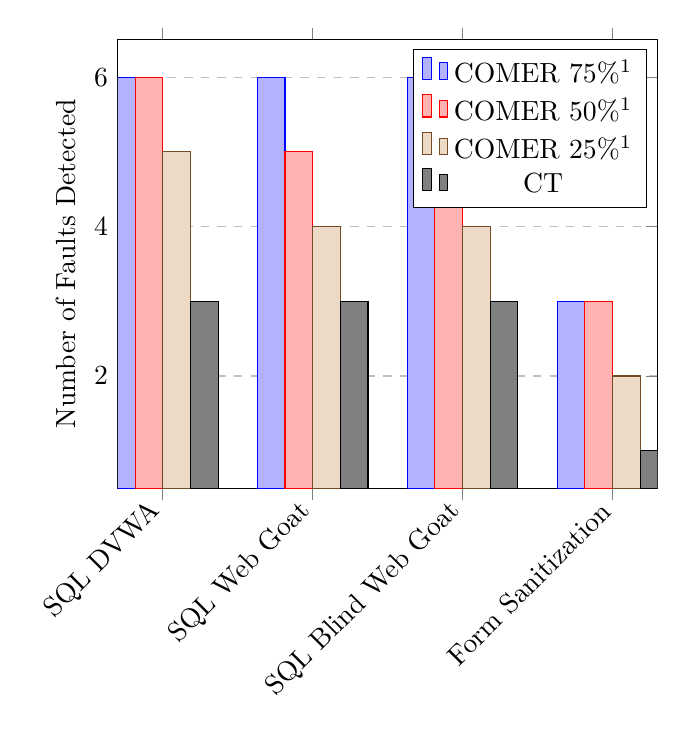
\begin{tikzpicture}
        \begin{axis}[
            ylabel={Number of Faults Detected},
            ybar=0pt,
            bar width=10pt,  % Adjusts th;e gap between bar groups
            ymajorgrids=true,
            grid style=dashed,
%             legend pos=north west,
            symbolic x coords={SQL DVWA, SQL Web Goat, SQL Blind Web Goat, Form Sanitization},
            xtick=data,
            x tick label style={rotate=45, anchor=east},
        ]

        \addplot coordinates {
            (SQL DVWA, 6)
            (SQL Web Goat, 6)
            (SQL Blind Web Goat, 6)
            (Form Sanitization, 3)
        };
        \addlegendentry{COMER 75\%$^1$}

        \addplot coordinates {
            (SQL DVWA, 6)
            (SQL Web Goat, 5)
            (SQL Blind Web Goat, 6)
            (Form Sanitization, 3)
        };
        \addlegendentry{COMER 50\%$^1$}

        \addplot coordinates {
            (SQL DVWA, 5)
            (SQL Web Goat, 4)
            (SQL Blind Web Goat, 4)
            (Form Sanitization, 2)
        };
        \addlegendentry{COMER 25\%$^1$}


        \addplot coordinates {
            (SQL DVWA, 3)
            (SQL Web Goat, 3)
            (SQL Blind Web Goat, 3)
            (Form Sanitization, 1)
        };
        \addlegendentry{CT}

        \end{axis}
    \end{tikzpicture}
    \caption{Number of Faults Detected for Different Injection Types. $^1$Percentage Corresponds to probability that MR approach will be selected.}
    \label{fig:faults}
\end{figure}

\begin{figure}[!t]
    \centering
    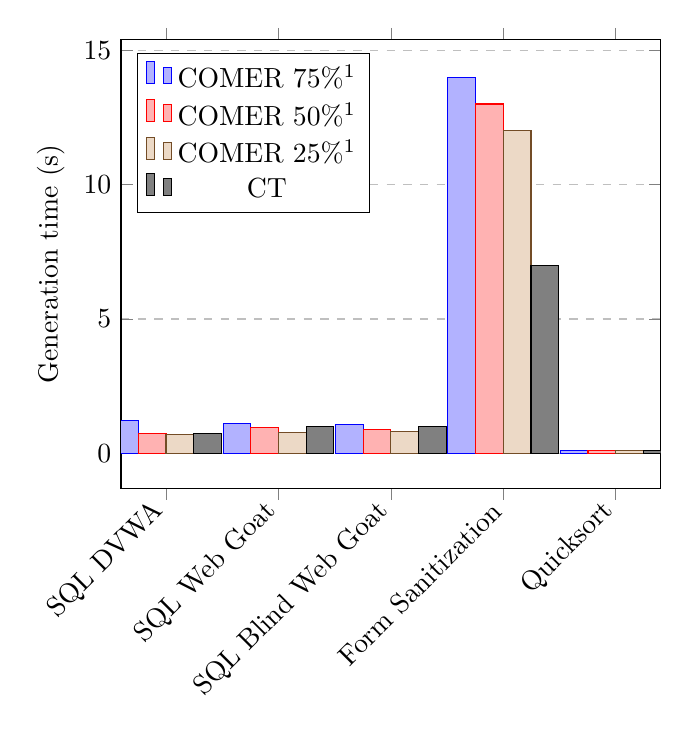
\begin{tikzpicture}
        \begin{axis}[
            ylabel={Generation time (s)},
            ybar=0pt,
            bar width=10pt,  % Adjusts th;e gap between bar groups
            ymajorgrids=true,
            grid style=dashed,
            legend pos=north west,
            symbolic x coords={SQL DVWA, SQL Web Goat, SQL Blind Web Goat, Form Sanitization, Quicksort},
            xtick=data,
            x tick label style={rotate=45, anchor=east},
        ]

        \addplot coordinates {
            (SQL DVWA, 1.24)
            (SQL Web Goat, 1.1)
            (SQL Blind Web Goat, 1.08)
            (Form Sanitization, 14)
            (Quicksort, 0.1)
        };
        \addlegendentry{COMER 75\%$^1$}

        \addplot coordinates {
            (SQL DVWA, 0.74)
            (SQL Web Goat, 0.96)
            (SQL Blind Web Goat, 0.89)
            (Form Sanitization, 13)
            (Quicksort, 0.1)
        };
        \addlegendentry{COMER 50\%$^1$}

        \addplot coordinates {
            (SQL DVWA, 0.7)
            (SQL Web Goat, 0.77)
            (SQL Blind Web Goat, 0.82)
            (Form Sanitization, 12)
            (Quicksort, 0.1)
        };
        \addlegendentry{COMER 25\%$^1$}


        \addplot coordinates {
            (SQL DVWA, 0.75)
            (SQL Web Goat, 1)
            (SQL Blind Web Goat, 1)
            (Form Sanitization, 7)
            (Quicksort, 0.1)
        };
        \addlegendentry{CT}

        \end{axis}
    \end{tikzpicture}
    \caption{Execution time in seconds for Different Injection Types. The \textit{Form Sanitization} takes longer time due to larger domain. $^1$Percentage Corresponds to probability that MR approach will be selected.}
    \label{fig:exec_time}
\end{figure}

\section{Discussion}

\subsection{COMER and Traditional CT}

To determine the efficiency of the approach, I compared the performance of the COMER framework with traditional CT methods in terms of test case generation efficiency. The results of the experiments demonstrate that the COMER framework is capable of generating test cases with a higher detection rate and about the same generation time compared to traditional CT methods. Different percentages of MR approach selection were tested to evaluate the impact of the MR approach on the results. The results indicate that the COMER framework can generate test cases more efficiently than traditional CT methods, especially when the MR approach is selected with a 50\% probability.

However, the number of test cases generated shown in Fig.~\ref{fig:test_cases} were higher than in the traditional CT approach, which may indicate that the COMER framework generates more test cases than necessary. This could potentially lead to increased resource utilization and inefficiency in the testing process. The results suggest that the COMER framework can be used as an effective alternative to traditional CT methods, but further optimization is needed to improve its efficiency. Currently, the utilization of MR approach with 50\% probability seems to be the most effective in terms of test case generation efficiency. It increases execution time by 2 times on average, but also increases the number of faults detected by 2 on average.

\subsection{COMER in Cybersecurity}

The results of the experiments demonstrate that the COMER framework is capable of generating test cases for testing Web Applications with a higher detection rate as shown in Fig.~\ref{fig:faults}, and about the same generation time compared to traditional CT methods, shown in Fig.~\ref{fig:exec_time}. The use of MRs allows the framework not only find potential for SQL injections, but also execute different kinds of SQL injections and other vulnerabilities. The results indicate that the COMER framework can be used to identify vulnerabilities in complex cybersecurity software more effectively than traditional CT methods. The framework's ability to generate test cases that target specific vulnerabilities makes it a valuable tool for cybersecurity professionals seeking to enhance the security of their applications.

\subsection{Standardization of COMER}

Due to the way this evaluation was implemented, it makes it easy to test software not covered by this thesis. This indicates that the COMER approach can be standardized into a framework or toolset for automated security testing. The framework's ability to efficiently identify vulnerabilities and generate test cases makes it a valuable tool for cybersecurity professionals seeking to enhance the security of their applications. The result of my work can be used as a foundation for developing a standardized framework that can be applied across various domains and applications.

\subsection{Systematic Generation of Metamorphic Relations}

The Metamorphic Relations (MRs) employed in this study were manually crafted for each specific test case. The process of fully automating MR generation remains a challenge due to the inherent complexity and domain knowledge it necessitates. The exploration of potential solutions, such as the utilization of Large Language Models (LLMs) or other methodologies, is out of the scope of this research. However, the results of this study demonstrate that the COMER framework has the potential to be extended to support the systematic generation of MRs for complex cybersecurity software.
